\documentclass[12pt,spanish,a4paper]{report}

% --- Paquetes Requeridos ---
\usepackage[utf8]{inputenc}
\usepackage[spanish,es-tabla]{babel}
\usepackage{geometry}
\geometry{a4paper, margin=2.5cm}
\usepackage{graphicx}
\usepackage{hyperref}
\usepackage{booktabs}
\usepackage{array}
\usepackage{tikz}
\usetikzlibrary{shapes.geometric, arrows, positioning, shadow, calc}
\usepackage{listings}
\usepackage{color}
\usepackage{amsmath}

% --- Configuración de Enlaces y PDF ---
\hypersetup{
    colorlinks=true,
    linkcolor=blue,
    filecolor=magenta,      
    urlcolor=cyan,
    pdftitle={Análisis del Reto - Primer Bimestre},
    pdfpagemode=FullScreen,
}

% --- Configuración de Código (Listings) ---
\definecolor{codegray}{rgb}{0.5,0.5,0.5}
\definecolor{codeblue}{rgb}{0.13,0.29,0.53}
\definecolor{backcolour}{rgb}{0.96,0.96,0.96}

\lstdefinestyle{mystyle}{
    backgroundcolor=\color{backcolour},   
    commentstyle=\color{codegray},
    keywordstyle=\color{codeblue}\bfseries,
    numberstyle=\tiny\color{codegray},
    stringstyle=\color{magenta},
    basicstyle=\ttfamily\footnotesize,
    breakatwhitespace=false,         
    breaklines=true,                 
    captionpos=b,                    
    keepspaces=true,                 
    numbers=left,                    
    numbersep=5pt,                  
    showspaces=false,                
    showstringspaces=false,
    showtabs=false,                  
    tabsize=2
}
\lstset{style=mystyle}

% --- Estilos TikZ para Diagramas ---
\tikzstyle{block} = [rectangle, draw, fill=blue!10, text width=7em, text centered, minimum height=3em, rounded corners]
\tikzstyle{cloud} = [ellipse, draw, fill=red!10, text width=5em, text centered, minimum height=2em]
\tikzstyle{db} = [cylinder, draw, shape border rotate=90, fill=green!10, text width=5em, text centered, minimum height=3.5em]
\tikzstyle{line} = [draw, -latex', thick]

% --- Portada ---
\begin{document}

\begin{titlepage}
    \centering
    \vspace*{1cm}
    
    {\scshape\LARGE Universidad Técnica Particular de Loja \par}
    \vspace{0.6cm}
    {\large Departamento de Ciencias de la Computación \par}
    {\large Carrera de Ingeniería en Ciencias de la Computación \par}
    \vspace{1.5cm}
    
    {\Large\bfseries PROYECTO BIMESTRAL\par}
    \vspace{0.5cm}
    {\huge\bfseries Análisis del Reto: Plataforma de Marketplace Mayorista B2B/B2C\par}
    \vspace{1.5cm}
    
    {\large\bfseries Autores: \\ David León \\ Víctor Mendoza \par}
    \vspace{0.8cm}
    {\large\bfseries Docente: \\ Ing. René Rolando Elizalde Solano \par}
    \vspace{0.8cm}
    {\large\bfseries Asignatura: \\ Plataformas Web \par}
    \vspace{0.8cm}
    {\large\bfseries Periodo y Paralelo: \\ Abril - Agosto 2026, Paralelo A \par}
    \vspace{1.5cm}
    
    {\large Loja - Ecuador \par}
    {\large Junio 2026 \par}
\end{titlepage}

% --- Sumario ---
\pdfbookmark{\contentsname}{toc}
\tableofcontents
\newpage

% --- Capítulo 1 ---
\chapter{Análisis del Reto}

\section{Introducción}
El sector de la distribución mayorista en el ámbito de negocios Business-to-Business (B2B) y Business-to-Consumer (B2C) se enfrenta a un proceso acelerado de transformación digital. Tradicionalmente, la intermediación comercial se ha basado en dinámicas presenciales o canales analógicos (llamadas telefónicas, hojas de pedido físicas), los cuales son propensos a ineficiencias de stock, errores humanos en facturación y demoras en los cobros. 

Para resolver esta brecha, se proyecta el desarrollo de una \textbf{Plataforma de Marketplace Mayorista B2B/B2C}. Este sistema digital unifica la interacción comercial entre tres actores principales:
\begin{itemize}
    \item \textbf{Empresas (Proveedores):} Entidades que ofertan mercancía al por mayor (lotes, pacas).
    \item \textbf{Vendedores Freelance:} Agentes comerciales independientes que representan a una o varias empresas para levantar pedidos en el territorio.
    \item \textbf{Tenderos o Clientes Finales:} Comercios minoristas locales que adquieren productos a través de la plataforma de forma autónoma o asistida.
\end{itemize}
El software propuesto facilita no solo la automatización del ciclo de venta y facturación, sino que gestiona dinámicamente un esquema de comisiones retenidas e incluye evaluaciones técnicas para habilitar vendedores certificados en nichos especializados (como la distribución farmacéutica).

\section{Problemática}
La gestión convencional de pedidos y logística comercial B2B adolece de problemas críticos que restringen el crecimiento de las empresas proveedoras y causan pérdidas a los comerciantes minoristas. Las principales problemáticas identificadas son:
\begin{enumerate}
    \item \textbf{Ventas Dobles y Desfase de Inventario:} La falta de sincronización del stock en tiempo real permite que dos vendedores consoliden pedidos sobre un lote único agotado, provocando anulaciones y descontento en los clientes.
    \item \textbf{Riesgo en la Cadena de Cobros:} Los pedidos mayoristas representan montos elevados. La ausencia de un canal seguro de pagos por adelantado (esquemas de 50\% o 100\%) expone a las empresas a impagos o cancelaciones tardías de mercancía ya despachada.
    \item \textbf{Informalidad en la Red de Ventas Freelance:} Al no existir un control automatizado de comisiones y entregas, el cálculo manual de la retribución de los vendedores freelance se vuelve complejo y opaco. Asimismo, las empresas corren riesgos al delegar la comercialización de productos regulados a personal sin la debida capacitación.
    \text{4. \textbf{Brecha Tecnológica (Analfabetismo Digital):}} El perfil demográfico del comerciante local (tendero) suele presentar resistencia al uso de plataformas complejas. Diseños con interfaces sobrecargadas o flujos extensos de compra incrementan la tasa de abandono de los pedidos.
\end{enumerate}

\section{Metodología o estrategia de desarrollo}
Para hacer frente a estas problemáticas y construir un producto robusto con entregas incrementales, se ha seleccionado el marco de trabajo ágil \textbf{Scrum} \cite{schwaber2002}. Esto permite iterar ágilmente sobre las especificaciones de requisitos funcionales y realizar demostraciones continuas al usuario final.

La estrategia tecnológica se basa en decisiones arquitectónicas enfocadas en la transaccionalidad, la escalabilidad y la personalización estética \cite{pressman2014}:
\begin{itemize}
    \item \textbf{Core de Desarrollo:} Arquitectura desacoplada basada en \textbf{Next.js} (React) con TypeScript para la interfaz frontend y \textbf{Django} (Python) con \textbf{Django REST Framework (DRF)} en el backend. Esta separación divide de forma limpia el desarrollo del cliente interactivo y las API de lógica de negocio del servidor.
    \item \textbf{Capa de Persistencia:} \textbf{PostgreSQL} como base de datos relacional. Su motor garantiza soporte nativo de transacciones ACID (Atomicity, Consistency, Isolation, Durability), indispensable para realizar bloqueos de fila (\textit{row locks}) que previenen la doble reserva de inventario de manera concurrente.
    \item \textbf{Acceso a Datos:} \textbf{Django ORM} para gestionar la comunicación con la base de datos PostgreSQL, facilitando la creación de modelos, migraciones de base de datos seguras y un panel administrativo integrado listo para producción.
    \item \textbf{Diseño de Interfaz:} \textbf{Vanilla CSS} empleando un sistema de variables y tokens globales. Se evita el uso de frameworks utilitarios como Tailwind CSS para mantener un control absoluto sobre el peso del bundle y garantizar una experiencia de usuario (UX) sumamente fluida con microanimaciones e interactividad adaptada a pantallas táctiles de dispositivos móviles.
\end{itemize}

\newpage

% --- Capítulo 2 ---
\chapter{Planificación y análisis}

\section{Análisis}
La plataforma web del Marketplace funciona bajo un modelo operativo de tres niveles comerciales con facturación integrada.
Las empresas proveedoras son las propietarias del catálogo mayorista y definen un monto mínimo de compra (entre \$60 y \$80) para hacer rentable el envío logístico. El sistema monetiza a través de un esquema doble: cobro de suscripción anual a los proveedores o aplicación de un porcentaje fijo (2\%) sobre el valor total de cada transacción finalizada.

El flujo de comisión para los vendedores independientes está integrado al ciclo de entrega. Cuando el vendedor registra una transacción, la comisión se calcula de acuerdo con los márgenes parametrizados por el proveedor. Dicha comisión permanece en estado "Retenida" en la base de datos hasta que el tendero confirma explícitamente haber recibido la mercancía, momento en el cual se libera la comisión para su respectiva transferencia, garantizando así la calidad del servicio.

\section{Requisitos funcionales}
A continuación, se tabulan los requisitos funcionales (RF) extraídos de la especificación técnica del proyecto:

\begin{table}[h!]
\centering
\small
\begin{tabular}{p{2cm} p{12cm}}
\toprule
\textbf{Código} & \textbf{Descripción del Requisito Funcional} \\
\midrule
\textbf{RF1.1} & Registro e inicio de sesión seguro con roles diferenciados: Administrador, Empresa (Proveedor), Vendedor Freelance y Tendero (Cliente). \\
\textbf{RF1.2} & Configuración empresarial del perfil de vendedor freelance requerido (Perfil General o Perfil Calificado). \\
\textbf{RF1.3} & Módulo de exámenes y certificaciones en línea para habilitar a vendedores freelance en perfiles calificados. \\
\textbf{RF2.1} & Visualización dinámica de catálogo mayorista orientado a paquetes cerrados, lotes y pacas. \\
\textbf{RF2.2} & Control y visualización del stock en tiempo real por cada almacén de proveedor. \\
\textbf{RF2.3} & Alertas y notificaciones automáticas ante niveles de stock inferiores al umbral de seguridad. \\
\textbf{RF2.4} & Sincronización del inventario mediante APIs o webhooks con ERPs o sistemas contables externos de los proveedores. \\
\textbf{RF3.1} & Compra directa autogestionada por Tenderos que cumplan con el monto mínimo. \\
\textbf{RF3.2} & Levantamiento de pedidos presencial por Vendedores Freelance a nombre de Tenderos. \\
\textbf{RF3.3} & Configuración dinámica por parte de las empresas de montos mínimos de compra. \\
\textbf{RF3.4} & Generación y envío automático de facturación detallada tras cada orden. \\
\textbf{RF4.1} & Pasarela de pagos integrada para abono de anticipo (50\%) o pago total (100\%). \\
\textbf{RF4.2} & Cálculo automatizado del porcentaje de comisión del freelance según márgenes establecidos. \\
\textbf{RF4.3} & Retención y liberación condicional de comisiones sujeta a la entrega efectiva del pedido. \\
\textbf{RF5.1} & Cobro automatizado de comisión transaccional (2\%) o membresía anual a los proveedores. \\
\bottomrule
\end{tabular}
\caption{Matriz de Requisitos Funcionales del Sistema.}
\label{tab:rf}
\end{table}

\newpage
\section{Requisitos no funcionales}
Los requisitos no funcionales (RNF) definen las restricciones de rendimiento, usabilidad, seguridad y plataforma tecnológica del sistema:

\begin{table}[h!]
\centering
\small
\begin{tabular}{p{2cm} p{12cm}}
\toprule
\textbf{Código} & \textbf{Descripción del Requisito No Funcional} \\
\midrule
\textbf{RNF1.1} & \textbf{Restricción de Canal:} El sistema se desplegará y optimizará inicialmente en formato de aplicación web interactiva (no nativa). \\
\textbf{RNF1.2} & \textbf{Integrabilidad:} Diseño modular basado en microservicios o API REST para facilitar enlaces contables fluidos. \\
\textbf{RNF2.1} & \textbf{Usabilidad Simplificada:} La UI para los Tenderos debe contar con tipografía de alta legibilidad, botones grandes de mínimo 48px y un flujo de compra rápido enfocado en reducir la fricción digital. \\
\textbf{RNF2.2} & \textbf{Flujo de Menor Clics:} El proceso desde la selección de artículos hasta el pago final debe completarse en un máximo de 3 pasos guiados. \\
\textbf{RNF3.1} & \textbf{Seguridad Transaccional:} Cumplimiento estricto de la norma PCI-DSS para transacciones mediante cifrado en Stripe. \\
\textbf{RNF3.2} & \textbf{Protección de Datos:} Cifrado irreversible (hashing con bcrypt) de credenciales del usuario en la persistencia. \\
\textbf{RNF4.1} & \textbf{Tiempo Real:} Actualización de inventario con latencia menor a 1.5 segundos ante transacciones concurrentes. \\
\textbf{RNF4.2} & \textbf{Escalabilidad:} El esquema relacional de PostgreSQL y los modelos de Django ORM deben diseñarse bajo estándares que permitan una transición directa a APIs móviles. \\
\bottomrule
\end{tabular}
\caption{Matriz de Requisitos No Funcionales del Sistema.}
\label{tab:rnf}
\end{table}

\section{Historias de Usuario / Casos de Uso}
A continuación se formulan historias de usuario prioritarias que guían el desarrollo de la plataforma:

\subsection*{Historia de Usuario 1: Registro de Pedido por Freelance}
\textbf{Como} Vendedor Freelance,\\
\textbf{Quiero} registrar un pedido a nombre de un Tendero local desde mi interfaz móvil,\\
\textbf{Para} agilizar su abastecimiento e incrementar mi registro de comisiones.\\
\textbf{Criterios de Aceptación:}
\begin{itemize}
    \item El freelance debe buscar y seleccionar al Tendero cliente mediante su código de local o nombre.
    \item La interfaz debe validar que el pedido supere el monto mínimo de compra del proveedor seleccionado.
    \item El pedido se crea con estado "Pendiente de Confirmación de Entrega".
\end{itemize}

\subsection*{Historia de Usuario 2: Compra Directa Adaptada para Tendero}
\textbf{Como} Tendero con bajo conocimiento digital,\\
\textbf{Quiero} realizar una compra directa desde un catálogo simple con botones amplios,\\
\textbf{Para} surtir mi negocio sin depender de una llamada telefónica o visita física.\\
\textbf{Criterios de Aceptación:}
\begin{itemize}
    \item Visualizar fotos de productos agrupadas por categorías claras.
    \item Agregar artículos con botones flotantes de ``+'' y ``-'' de gran escala.
    \item Visualizar el resumen final con el cobro del 50\% inicial de manera simplificada en una sola pantalla.
\end{itemize}

\subsection*{Historia de Usuario 3: Creación de Test de Certificación}
\textbf{Como} Administrador de Empresa Proveedora de Productos Calificados (ej. Farmacéuticos),\\
\textbf{Quiero} diseñar un examen interactivo de certificación dentro de la plataforma,\\
\textbf{Para} garantizar que solo los vendedores freelance aprobados distribuyan mi stock de medicamentos.\\
\textbf{Criterios de Aceptación:}
\begin{itemize}
    \item Formulario para ingresar preguntas de opción múltiple con puntaje asignado.
    \item Establecer la nota mínima de aprobación (ej. 80\%).
    \item Los freelancers reprobados son bloqueados temporalmente para aplicar a la distribución de esa empresa.
\end{itemize}

\section{Sprint}
La planificación técnica de implementación se segmenta en dos Sprints iniciales de dos semanas cada uno:

\begin{enumerate}
    \item \textbf{Sprint 1: Inicialización y Core Arquitectónico}
    \begin{itemize}
        \item Definición de la estructura de carpetas en el cliente Next.js y en el backend Django.
        \item Diseño e implementación de modelos Django y migraciones en PostgreSQL.
        \item Configuración de la autenticación mediante tokens en Django REST Framework.
        \item Creación de comandos de semilla (fixtures/seeders) en Django para usuarios y perfiles iniciales.
        \item Creación del Layout CSS global con variables de diseño premium.
    \end{itemize}
    \item \textbf{Sprint 2: Catálogo Mayorista y Sistema de Pedidos}
    \begin{itemize}
        \item Implementación de vistas de catálogos mayoristas adaptables en Next.js.
        \item Integración de la API de Django REST Framework con el cliente Next.js.
        \item Integración de cobros de Stripe en las vistas del backend Django.
        \item Lógica de retención de comisiones y panel de verificación de entregas en Django.
        \item Pruebas funcionales concurrentes para validar la integridad en la reducción de stock.
    \end{itemize}
\end{enumerate}

\newpage
\section{Diagramas: Casos de Uso del Sistema - Preguntas y respuesta al diagrama}

El comportamiento y los requisitos funcionales del sistema se modelan mediante un diagrama de casos de uso, el cual detalla la interacción de los actores (tanto usuarios de la plataforma como sistemas externos) con las funcionalidades principales de la plataforma. A continuación se presenta el diagrama correspondiente:

\begin{figure}[h!]
\centering
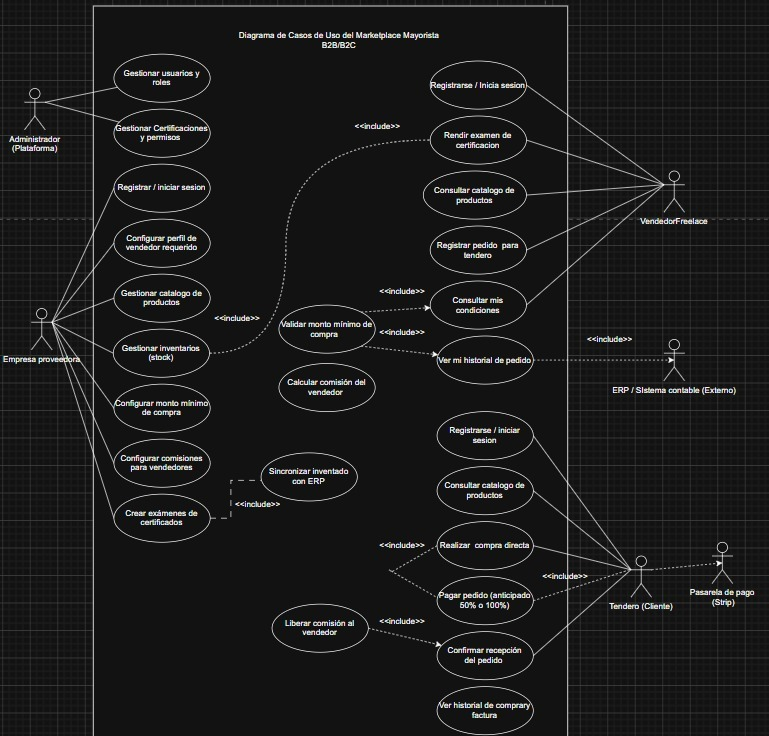
\includegraphics[width=0.95\textwidth]{caso_de_uso.jpg}
\caption{Diagrama de Casos de Uso del Marketplace Mayorista B2B/B2C.}
\label{fig:use_cases}
\end{figure}

\subsection*{Preguntas y Respuestas al Diseño del Diagrama}

\begin{enumerate}
    \item \textbf{¿Cómo se gestiona el inventario de forma segura ante pedidos concurrentes?}
    \textbf{Respuesta:} Se utiliza PostgreSQL bajo aislamiento de transacciones o bloqueos pesimistas selectivos mediante el uso de \lstinline{select_for_update()} en el ORM de Django dentro de una transacción atómica (\lstinline{@transaction.atomic}). Al iniciar la transacción de compra, Django ORM bloquea la fila del producto en evaluación, verificando que el stock sea suficiente antes de proceder con el débito y la creación del pedido. Si el stock no cumple, la transacción realiza un rollback completo.
    \item \textbf{¿De qué manera interactúan las cuentas de usuarios con perfiles de especialización?}
    \textbf{Respuesta:} La tabla o modelo \lstinline{User} centraliza la autenticación en Django (extendiendo la clase \lstinline{AbstractUser}). Dependiendo del valor asignado al campo \lstinline{role} (\lstinline{EMPRESA}, \lstinline{VENDEDOR_FREELANCE}, \lstinline{TENDERO}, \lstinline{ADMIN}), el backend enlaza la cuenta a su perfil correspondiente en \lstinline{CompanyProfile} o \lstinline{FreelanceProfile} a través de relaciones de tipo \lstinline{OneToOneField}.
    \item \textbf{¿Cómo se restringe la venta de un producto que requiere perfil calificado?}
    \textbf{Respuesta:} Cuando un freelance intenta levantar un pedido de un proveedor con certificaciones activas, el servidor de Django ejecuta un query que verifica la existencia de un registro de aprobación con \lstinline{passed = True} en el modelo \lstinline{CertificationAttempt} para el \lstinline{CertificationTest} correspondiente a dicha empresa. Si no se cumple la condición, el backend retorna una excepción de tipo \lstinline{PermissionDenied}.
    \item \textbf{¿Qué rol cumple el actor externo "Pasarela de pagos (Stripe)" y cómo se relaciona con el caso de uso "Pagar pedido"?}
    \textbf{Respuesta:} El actor "Pasarela de pagos (Stripe)" es un sistema externo que interactúa directamente con el caso de uso "Pagar pedido (anticipado 50\% o 100\%)". Tras recibir la orden de pago desde el frontend en Next.js, Django gestiona la sesión de Stripe y, una vez que el usuario ingresa sus datos financieros en el portal seguro de Stripe, esta pasarela notifica el éxito del cobro al backend para validar y procesar la orden.
    \item \textbf{¿Cómo interactúa el caso de uso "Sincronizar inventario con ERP" con el sistema de la empresa proveedora?}
    \textbf{Respuesta:} Este caso de uso permite que los inventarios físicos de la empresa proveedora se sincronicen bidireccionalmente. Cuando la empresa realiza cambios en su stock local a través de su ERP externo, este se comunica con el backend del Marketplace mediante la API REST expuesta en Django, garantizando que el catálogo de productos muestre existencias reales de forma automática.
\end{enumerate}

\newpage
\section{Diagrama de componentes}
El diagrama de componentes detalla la arquitectura modular del software y la comunicación orientada al cliente-servidor:

\begin{figure}[h!]
\centering
\begin{tikzpicture}[node distance=2.2cm, auto, every node/.style={font=\sffamily\small}]
    % Capas
    \node [block, fill=orange!15] (ui) {\textbf{Capa de Presentación} \\ (Next.js Client, Vanilla CSS, Responsive UI)};
    \node [block, fill=blue!15, below=of ui] (api) {\textbf{Capa de Negocio} \\ (Django REST API, Auth Token, Controllers)};
    \node [db, below=of api] (db) {\textbf{Capa de Datos} \\ (PostgreSQL \& Django ORM)};
    \node [block, fill=red!15, right=of api, xshift=2.5cm] (ext) {\textbf{Servicios Externos} \\ (Stripe SDK, ERP Webhooks)};

    % Enlaces
    \draw [line, <->] (ui) -- node[right] {HTTP Request / JSON} (api);
    \draw [line, <->] (api) -- node[right] {Django ORM Queries} (db);
    \draw [line, ->] (api) -- node[above] {API Calls} (ext);
\end{tikzpicture}
\caption{Diagrama de Componentes de la Aplicación.}
\label{fig:components}
\end{figure}

\section{Arquitectura lógica y física (propuesta)}
La propuesta arquitectónica garantiza una alta disponibilidad física y un acoplamiento débil a nivel lógico:

\subsection*{Arquitectura Lógica}
Estructurada bajo un patrón de arquitectura desacoplada frontend/backend:
\begin{enumerate}
    \item \textbf{Capa de Interfaz de Usuario (Frontend):} Implementada en Next.js (React), encargada de renderizar las vistas dinámicas de forma responsiva y consumir los endpoints de la API REST backend mediante peticiones asíncronas.
    \item \textbf{Capa de API y Backend (Lógica de Negocio):} Construida en Django utilizando Django REST Framework (DRF). Maneja la validación de montos mínimos, cálculo de comisiones, autenticación por tokens (JWT o SimpleJWT), control de acceso multi-rol y la comunicación con servicios externos.
    \item \textbf{Capa de Persistencia:} Gestionada por el ORM de Django, que interactúa directamente con PostgreSQL. Ofrece seguridad integrada ante inyecciones de código y asegura la integridad transaccional mediante decoradores y transacciones atómicas nativas.
\end{enumerate}

\subsection*{Arquitectura Física}
El esquema físico propuesto aprovecha entornos especializados para frontend y backend:
\begin{itemize}
    \item \textbf{Hospedaje Frontend:} \textbf{Vercel} o Netlify para alojar y servir la aplicación Next.js de forma estática y optimizada.
    \item \textbf{Hospedaje Backend:} Servidores basados en contenedores o PaaS como \textbf{Render}, Heroku o AWS Elastic Beanstalk para ejecutar la aplicación de Django bajo un servidor WSGI/ASGI (como Gunicorn/Uvicorn).
    \item \textbf{Base de Datos Hospedada:} Instancia de PostgreSQL gestionada en la nube mediante \textbf{Neon.tech} o Supabase.
    \item \textbf{Pasarelas y Servicios:} Servidores de Stripe para los pagos electrónicos.
\end{itemize}

\section{Prototipo de pantallas no funcional}

El diseño de la interfaz gráfica prioriza la sencillez, la legibilidad y la experiencia visual premium (con un esquema de colores oscuro, tipografía legible y microinteracciones claras) para reducir la fricción digital en los minoristas y ofrecer herramientas eficientes a las empresas y vendedores. A continuación, se detallan los prototipos de pantalla desarrollados para cada flujo operativo:

\subsection{Flujo de la Tienda Online (Vista del Tendero / Cliente)}
Representa la experiencia de compra directa adaptada para el tendero local, facilitando un proceso sin fricciones y guiado en todo momento.

\begin{figure}[h!]
\centering
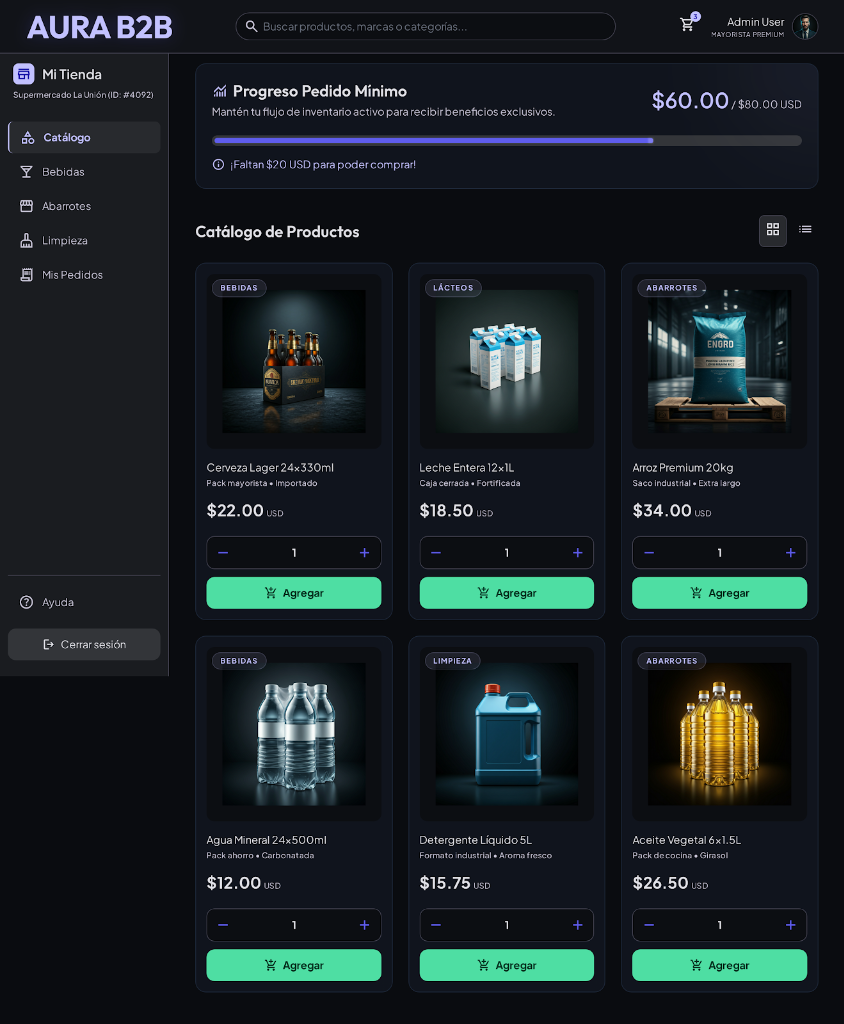
\includegraphics[width=0.85\textwidth]{proto_tienda_catalogo.png}
\caption{Prototipo 1: Catálogo de Productos y barra de progreso del monto mínimo de compra.}
\label{fig:proto_catalogo}
\end{figure}

\begin{figure}[h!]
\centering
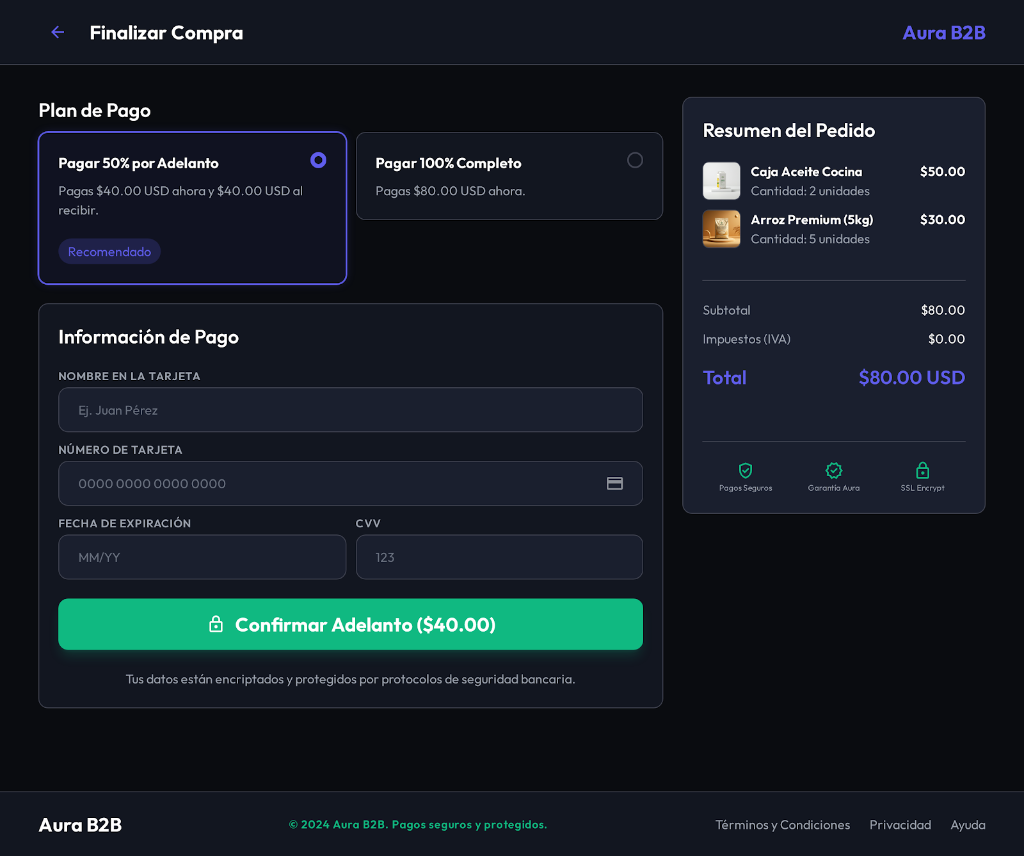
\includegraphics[width=0.85\textwidth]{proto_tienda_pago.png}
\caption{Prototipo 2: Pantalla de finalización de compra (Checkout) con opciones de pago del 50\% o 100\%.}
\label{fig:proto_pago}
\end{figure}

\begin{figure}[h!]
\centering
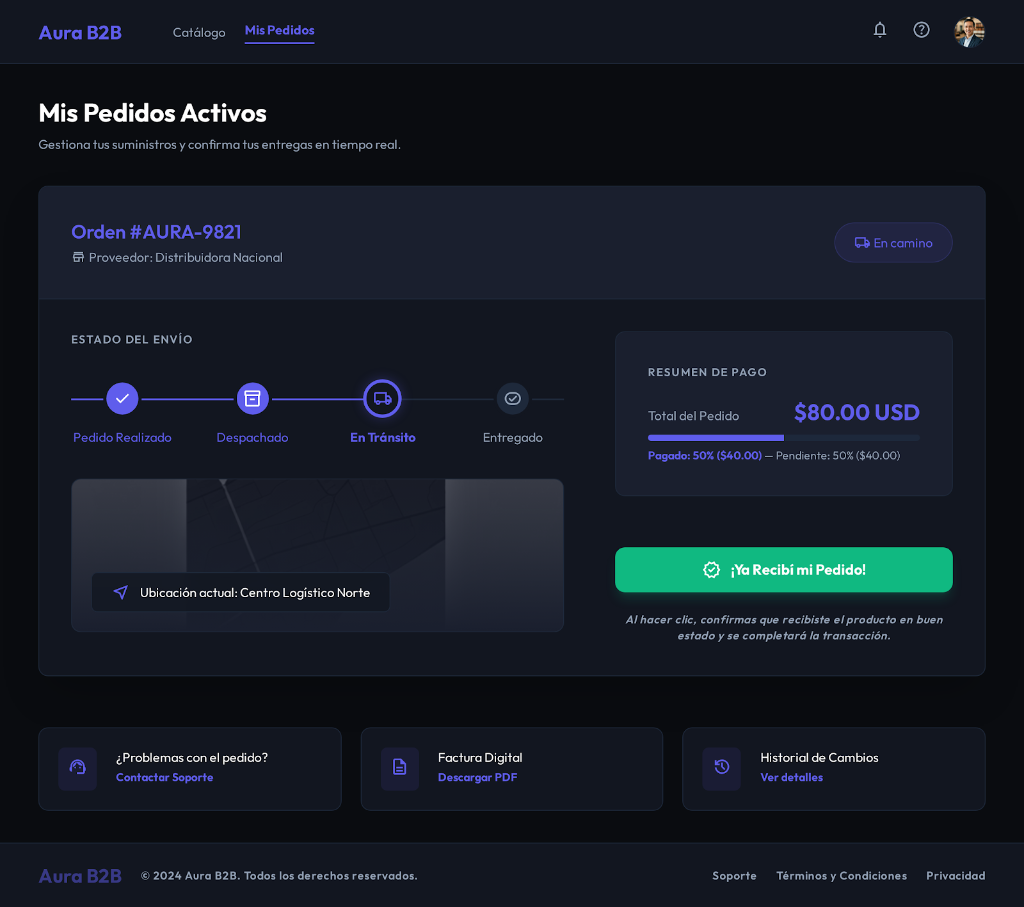
\includegraphics[width=0.85\textwidth]{proto_tienda_pedido.png}
\caption{Prototipo 3: Rastreo activo de pedidos y confirmación de recepción en tiempo real.}
\label{fig:proto_pedido}
\end{figure}

\newpage
\subsection{Flujo del Vendedor Freelance (Dashboard de Ventas)}
Consola de administración donde el vendedor freelance registra sus pedidos a nombre de tenderos, valida sus comisiones y visualiza el estado de sus certificaciones activas.

\begin{figure}[h!]
\centering
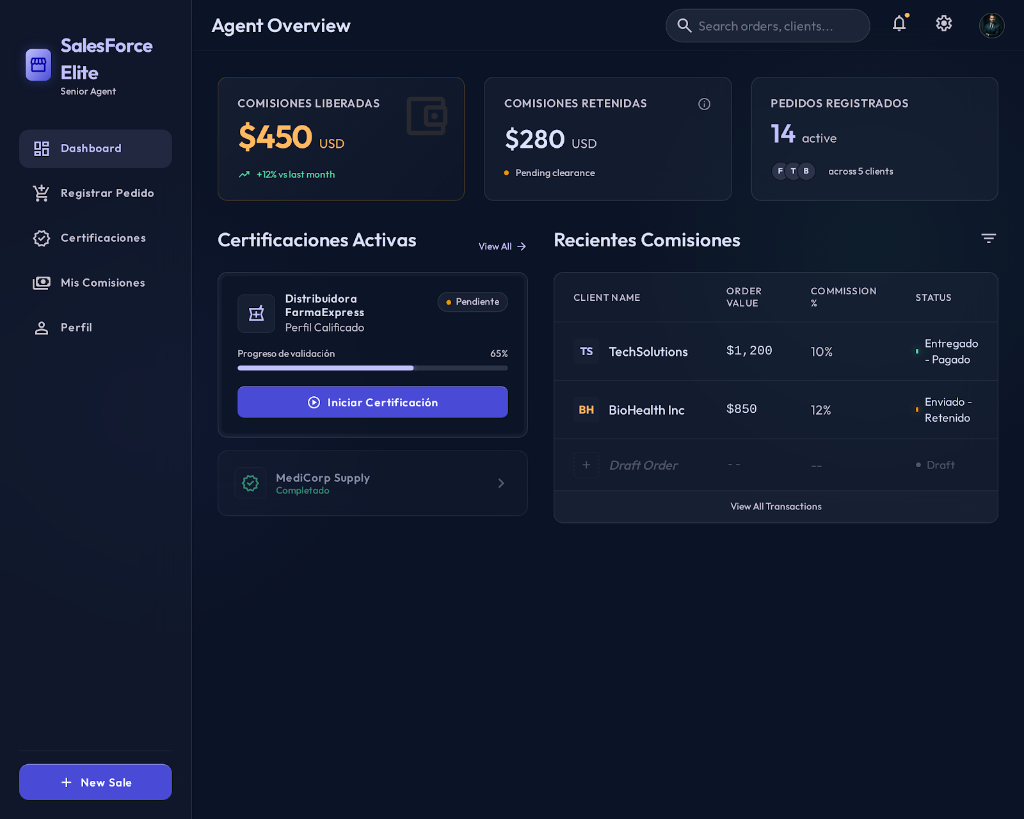
\includegraphics[width=0.85\textwidth]{proto_dashboard_freelance.png}
\caption{Prototipo 4: Dashboard general del Agente Freelance con comisiones y estado de certificaciones.}
\label{fig:proto_dashboard}
\end{figure}

\subsection{Flujo de la Empresa Proveedora (Panel de Control de Distribución)}
Panel administrativo para la empresa donde se configura el monto mínimo de compra, se confirman pedidos y se monitorean las alertas automáticas de stock.

\begin{figure}[h!]
\centering
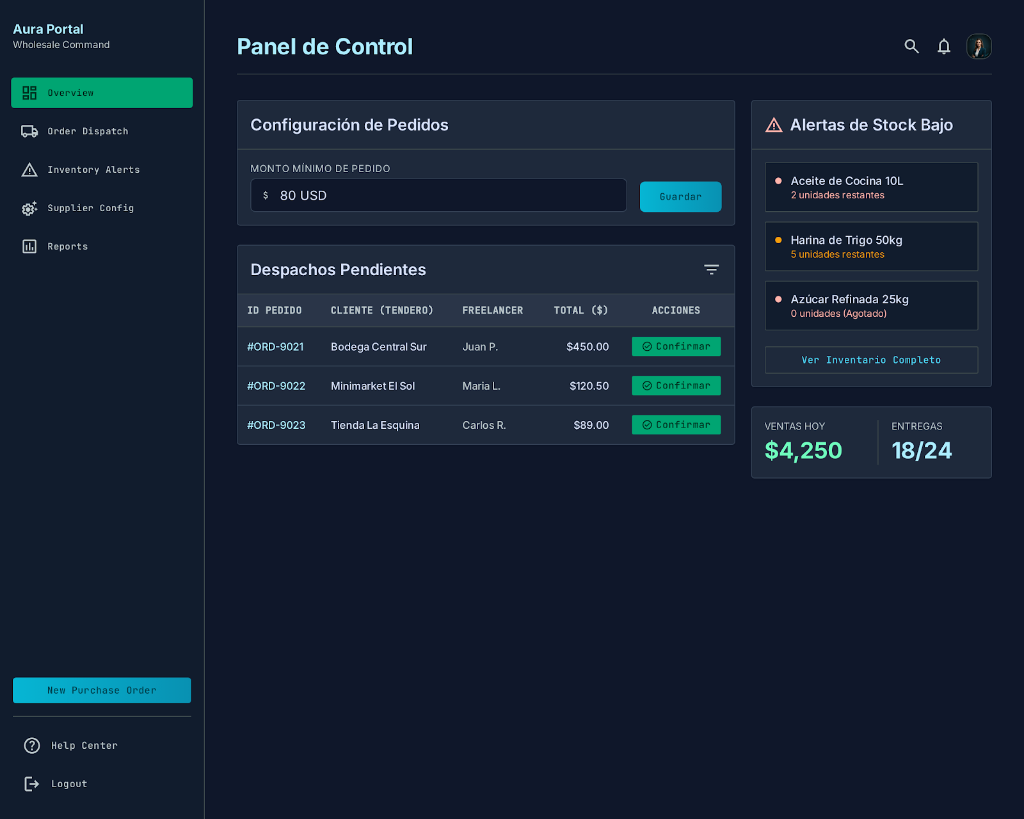
\includegraphics[width=0.85\textwidth]{proto_panel_proveedor.png}
\caption{Prototipo 5: Panel de Control de Administración del Proveedor.}
\label{fig:proto_panel}
\end{figure}

% --- Bibliografía ---
\begin{thebibliography}{9}
\bibitem{nextjs} Vercel. Next.js Documentation. 2026. \url{https://nextjs.org/docs}
\bibitem{django} Django Software Foundation. Django Documentation. 2026. \url{https://docs.djangoproject.com}
\bibitem{django_rest_framework} Encode Collaborative. Django REST Framework Documentation. 2026. \url{https://www.django-rest-framework.org}
\bibitem{postgresql} The PostgreSQL Global Development Group. PostgreSQL 16 Documentation. 2026. \url{https://www.postgresql.org/docs/16/index.html}
\bibitem{stripe} Stripe. Stripe API Reference. 2026. \url{https://stripe.com/docs/api}
\bibitem{pressman2014} Pressman, Roger S. Software Engineering: A Practitioner's Approach. McGraw-Hill Education, 8th edition, 2014.
\bibitem{schwaber2002} Schwaber, Ken and Beedle, Mike. Agile Software Development with Scrum. Prentice Hall, 2002.
\end{thebibliography}

\end{document}
